\documentclass{standalone}
\usepackage{tikz}
\usetikzlibrary{arrows.meta}

\begin{document}

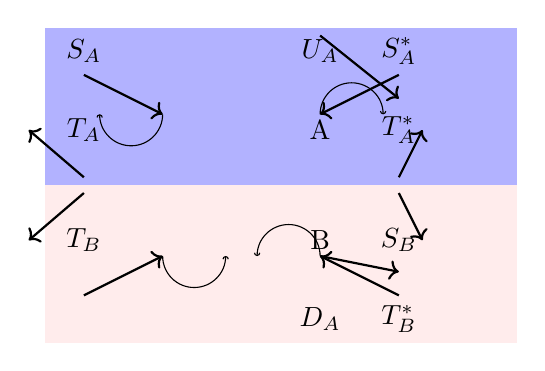
\begin{tikzpicture}[auto,
    every node/.style={inner sep=0pt},
    small arrow/.style={-Straight Barb, shorten >=1pt}
]

% Background color for the layers
\fill[blue!30] (0,0) rectangle (6,2);
\fill[pink!30] (0,0) rectangle (6,-2);

% Nodes for the labels
\node at (0.5,0.7) {$T_A$};
\node at (4.5,0.7) {$T_A^*$};
\node at (0.5,1.7) {$S_A$};
\node at (4.5,1.7) {$S_A^*$};
\node at (3.5,1.7) {$U_A$};
\node at (3.5,0.7) {A};

\node at (3.5,-0.7) {B};
\node at (3.5,-1.7) {$D_A$};
\node at (0.5,-0.7) {$T_B$};
\node at (4.5,-0.7) {$S_B$};
\node at (4.5,-1.7) {$T_B^*$};

% Arrows for the optical depths
\draw[->,thick] (0.5,0.1) -- (-0.2,0.7);
\draw[->,thick] (4.5,0.1) -- (4.8,0.7);
\draw[->,thick] (0.5,-0.1) -- (-0.2,-0.7);
\draw[->,thick] (4.5,-0.1) -- (4.8,-0.7);

% Arrows for the fluxes
\draw[->,thick] (3.5,1.9) -- (4.5,1.1);
\draw[->,thick] (3.5,-0.9) -- (4.5,-1.1);

% Arrows for the scattering and transmission functions
\draw[->,thick] (0.5,1.4) -- (1.5,0.9);
\draw[->,thick] (4.5,1.4) -- (3.5,0.9);
\draw[->,thick] (4.5,-1.4) -- (3.5,-0.9);
\draw[->,thick] (0.5,-1.4) -- (1.5,-0.9);

% Arcs for the scattering and transmission directions
\draw[-{Arc Barb[scale=0.5]}] (1.5,0.9) arc (0:-180:0.4);
\draw[-{Arc Barb[scale=0.5]}] (3.5,-0.9) arc (0:180:0.4);
\draw[-{Arc Barb[scale=0.5]}] (3.5,0.9) arc (180:0:0.4);
\draw[-{Arc Barb[scale=0.5]}] (1.5,-0.9) arc (-180:0:0.4);

\end{tikzpicture}

\end{document}